\section{Offline Synthesis}\label{sec:reactive_gait_synthesis}
% The offline synthesis module 
% generates a strategy 
% that enables the robot
% to reach desired goal waypoints over all predefined terrain states.
% As shown in Fig.~\ref{fig:combined_offline_online}(a),
% this module takes in
% a set of request goals and
% a set of possible terrain states from prior knowledge of the workspace. In addition, a set of locomotion gaits is also provided by the user. After discretizing the local environment and characterizing the terrains in Sec.~\ref{sec:preliminaries_abstraction}, we first solve a gait-fixed MICP problem to determine the feasibility of each potential skill given the locomotion gaits
% (Sec.~\ref{sec:motion_primitive}), and then encode all feasible transitions as skills in a specification
% (Sec.~\ref{sec:spec_gen}).
% If the specification is realizable, we generate a strategy for online execution.
% Otherwise, we leverage a repair process to suggest new robot skills, utilize the gait-free MICP planner to check the feasibility of the suggested skills, and eventually make the specification realizable
% (Sec.~\ref{sec:symbolic_repair}).
%%%% Fig4. System overview %%%%
\begin{figure*}[ht]
    \centering
    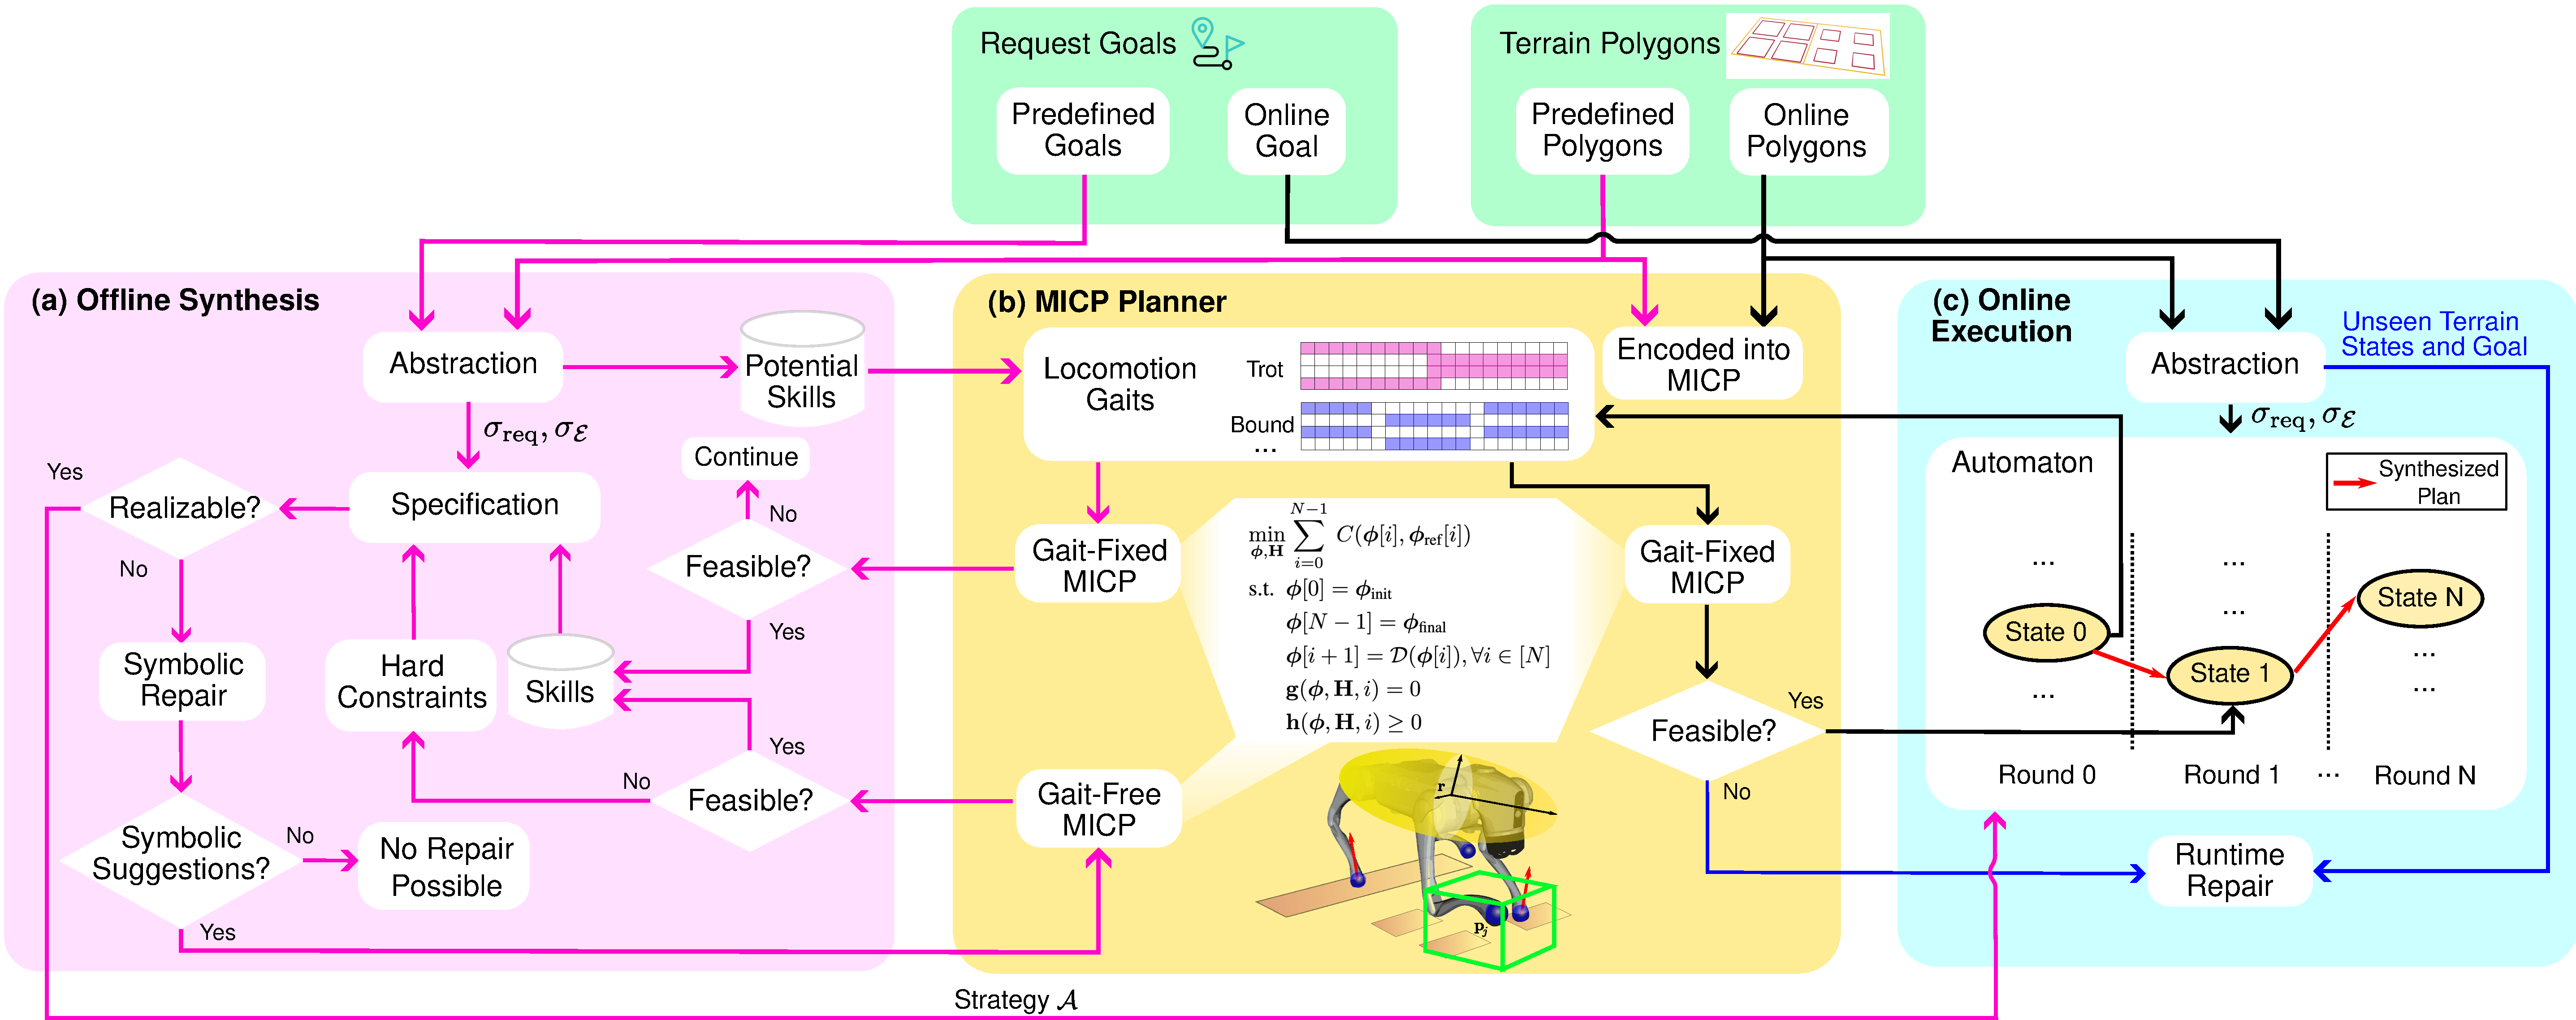
\includegraphics[width=\linewidth]{combined_offline_online_v2.pdf}
    \caption{System overview.  
    % for offline synthesis and online execution. 
    During offline synthesis (pink arrows), an initial set of locomotion gaits is provided, and symbolic skills are iteratively generated by solving the MICP. When the task specifications are unrealizable, a symbolic repair is triggered to seek missing skills.
    During the online execution (black arrows), MICP is solved again taking online terrain segments and the symbolic state only advances when a solution is found.
    % During online execution (black arrows), the MICP is solved again using incoming terrain segments, and the symbolic state is advanced only once a valid solution is obtained. 
    A runtime repair (blue arrows) is initiated if a solving failure occurs, 
    or an unseen terrain or request goal is encountered.
    }
    \label{fig:combined_offline_online}
    \vspace{-0.1in}
\end{figure*}
%%%%%%%%%%%%%%%%%%%%%%%%%%%%%%%%%%%

The offline synthesis module builds a strategy that allows the robot to reach local request goals under predefined terrain conditions. As shown in Fig.~\ref{fig:combined_offline_online}(a), the module takes in local request goals $\mathcal{G}_{\textrm{local}}$, terrain polygons $\mathcal{P}_{\text{pre}}$ from prior maps, and a set of locomotion gaits $\mathcal{L}$ specified by the user.
We first apply the inverse grounding function $\inversegrounding$ to discretize the local environment, deriving a set of candidate request states $\inpstatesrequestposs \subseteq \inpstatesrequest$ from the local request goals and mapping the predefined terrain polygons into possible terrain states $\inpstatesterrainexprposs \subseteq \inpstatesterrain$.
Afterward, we evaluate the feasibility of each candidate skill using a gait-fixed MICP formulated with the provided locomotion gaits (Sec.~\ref{sec:motion_primitive}), and record all feasible transitions as symbolic skills in the specification (Sec.~\ref{sec:spec_gen}).
To improve efficiency, a high-level manager then generates partial evaluations of the encoded specifications. Whenever one of these partial evaluations is deemed unrealizable, a repair mechanism is invoked: it proposes additional symbolic skills, whose feasibility is validated through gait-free MICP. This process ensures that the specification ultimately becomes realizable (Sec.~\ref{sec:manager_and_repair}).
% We first 
% use the inverse grounding function $\inversegrounding$ to 
% discretize the local environment,
% obtain
% a set of possible
% request states $\inpstatesrequestposs \subseteq \inpstatesrequest$
% from the local request goals,
% and characterize the predefined set of terrain polygons into a set of possible terrain states $\inpstatesterrainexprposs \subseteq \inpstatesterrain$.
% Next, 
% we solve a gait-fixed MICP problem to determine the feasibility of each potential skill given the locomotion gaits
% (Sec.~\ref{sec:motion_primitive}), and then encode all feasible transitions as skills in a specification
% (Sec.~\ref{sec:spec_gen}).
% Next,
% we use a high-level manager to 
% generate partial evaluations of the encoded specifications
% for efficient synthesis.
% If any partial evaluation is unrealizable, 
% we leverage a repair process to suggest new symbolic-level robot skills 
% and a gait-free MICP to verify the feasibility of the suggested skills, 
% eventually making the specification realizable
% (Sec.~\ref{sec:manager_and_repair}).


% The reactive synthesis process has two phases: offline synthesis and online execution. 
% We begin by introducing the essential specifications that define our terrain-adaptive locomotion problem. The objective is to construct a high-level robot gait and keyframe transition strategy by solving a two-player game between the gait planner and its possibly adversarial environment. The Linear Temporal Logic (LTL) specifications are designed by human experts, who provide logical rules that guide the planning process. It is nothworthy that the specification design is not unique and may vary according to expert input.

% Add a mapping function from the discrete state to the continuous state?

% \subsection{Motion Primitives to Robot Skills}\label{sec:motion_primitive}
\subsection{Locomotion Gait and Feasibility Checking via MICP}\label{sec:motion_primitive} 
We assume each locomotion gait $L$ is characterized by a contact sequence $\mathcal{G}$ and its associated time durations $T$, formally written as $L = \mathcal{M}(\mathcal{G}, T)$. Each skill is tied to a distinct locomotion gait, which dictates how the robot executes motion at the continuous level.
As illustrated in Fig.~\ref{fig:combined_offline_online}(a), since the offline phase has access to the complete set of request states $\inpstatesrequestposs$ and terrain states $\inpstatesterrainexprposs$, we can systematically enumerate all possible symbolic skills that enable navigation across the different local environments. The feasibility of each skill is then evaluated through gait-fixed MICP using the given locomotion gaits.
% We assume each locomotion gait comes with a contact sequence $\mathcal{G}$ and corresponding time durations $T$. Therefore, we define the locomotion gait as $L = \mathcal{M}(\mathcal{G}, T)$. Each skill is assumed to have a unique locomotion gait to determine how the robot moves at the continuous level. 
% As shown in Fig.~\ref{fig:combined_offline_online}(a), since all the possible request goals $\inprequest$ and terrain states $\inpterrain$ are predefined during the offline phase, it is straightforward to first identify all the potential skills at the symbolic level that allow the robots to move freely in all possible local environments. 
In most examples shown in this paper, we assume the robot is only allowed to move horizontally and vertically by one cell and we show diagonal movements and heading angle change in Sec.~\ref{sec:extension}.
% Then, 
% we formulate a MICP problem that
% each MICP solve can 
% takes in 

Then the next critical step is to find whether there exists a locomotion gait for each skill to be physically feasible.
We leverage mixed-integer convex programming (MICP) to check the physical feasibility given a set of predefined locomotion gaits, and only use the feasible one as robot skills to synthesize robot strategies. The MICP problem takes in
the centroidal states $\inpcen$ from the precondition and postcondition of the skill as its initial and final conditions, which are located at the center of each abstracted cell. A set of homogeneous, predefined terrain polygons are considered in the MICP as steppable regions corresponding to the terrain states $\inpterrain$ involved in the precondition. Lastly, the contact information $\mathcal{G}$ and $T$ is provided by the selected locomotion gait $L$. Fig.~\ref{fig:mip_go2} shows the maneuver of the quadruped robot Go2 after solving the MICP problem corresponding to skill $a_0$ in Example~\ref{example:1} with a one-second trotting locomotion gait. The generic MICP problem considered in this work can formulated as:
    \begin{subequations}\label{ocp:mip_general}
    \begin{alignat}{2}
        \nonumber &\underset{\vg \phi, \v H}{\min} && \sum_{i = 0}^{N-1} \hspace{2pt} C(\vg \phi[i], \vg \phi_{\text{ref}}[i])\\
        & \text{s.t. } && \vg \phi[0] = \vg \phi_{\text{init}} \\& && \vg \phi[N-1] = \vg \phi_{\text{final}} \\
     & &&  \vg \phi[i+1] = \mathcal{D}(\vg \phi[i]), \forall i \in \range{N} \\
        & && \v g(\vg \phi, \v H, i) = 0 \\
        & && \v h(\vg \phi, \v H, i) \geq 0
    \end{alignat}
\end{subequations}
where the decision variables $\vg \phi$ denote the continuous variables and $\v H$ indicate the binary variables across the entire $N$ timesteps. For any natural number $n \in \naturals$, we denote the set $\{0, \dots, n-1\}$ as $\range{n}$. \revised{The function $\mathcal{D}(\cdot)$ encodes the discrete-time system dynamics that propagate the continuous state $\vg \phi[i]$ to $\vg \phi[i+1]$; the specific dynamics used in this work are detailed in Eq.~(\ref{eq:dynamics}).} The general equality constraints $\v g(\cdot)$ and inequality constraints $\v h(\cdot)$ are incorporated and activated at certain time stamp $i$. The cost function depends on both the continuous variables $\vg \phi$ and a reference trajectory $\vg \phi_{\text{ref}}$.

\begin{figure}
    \centering
    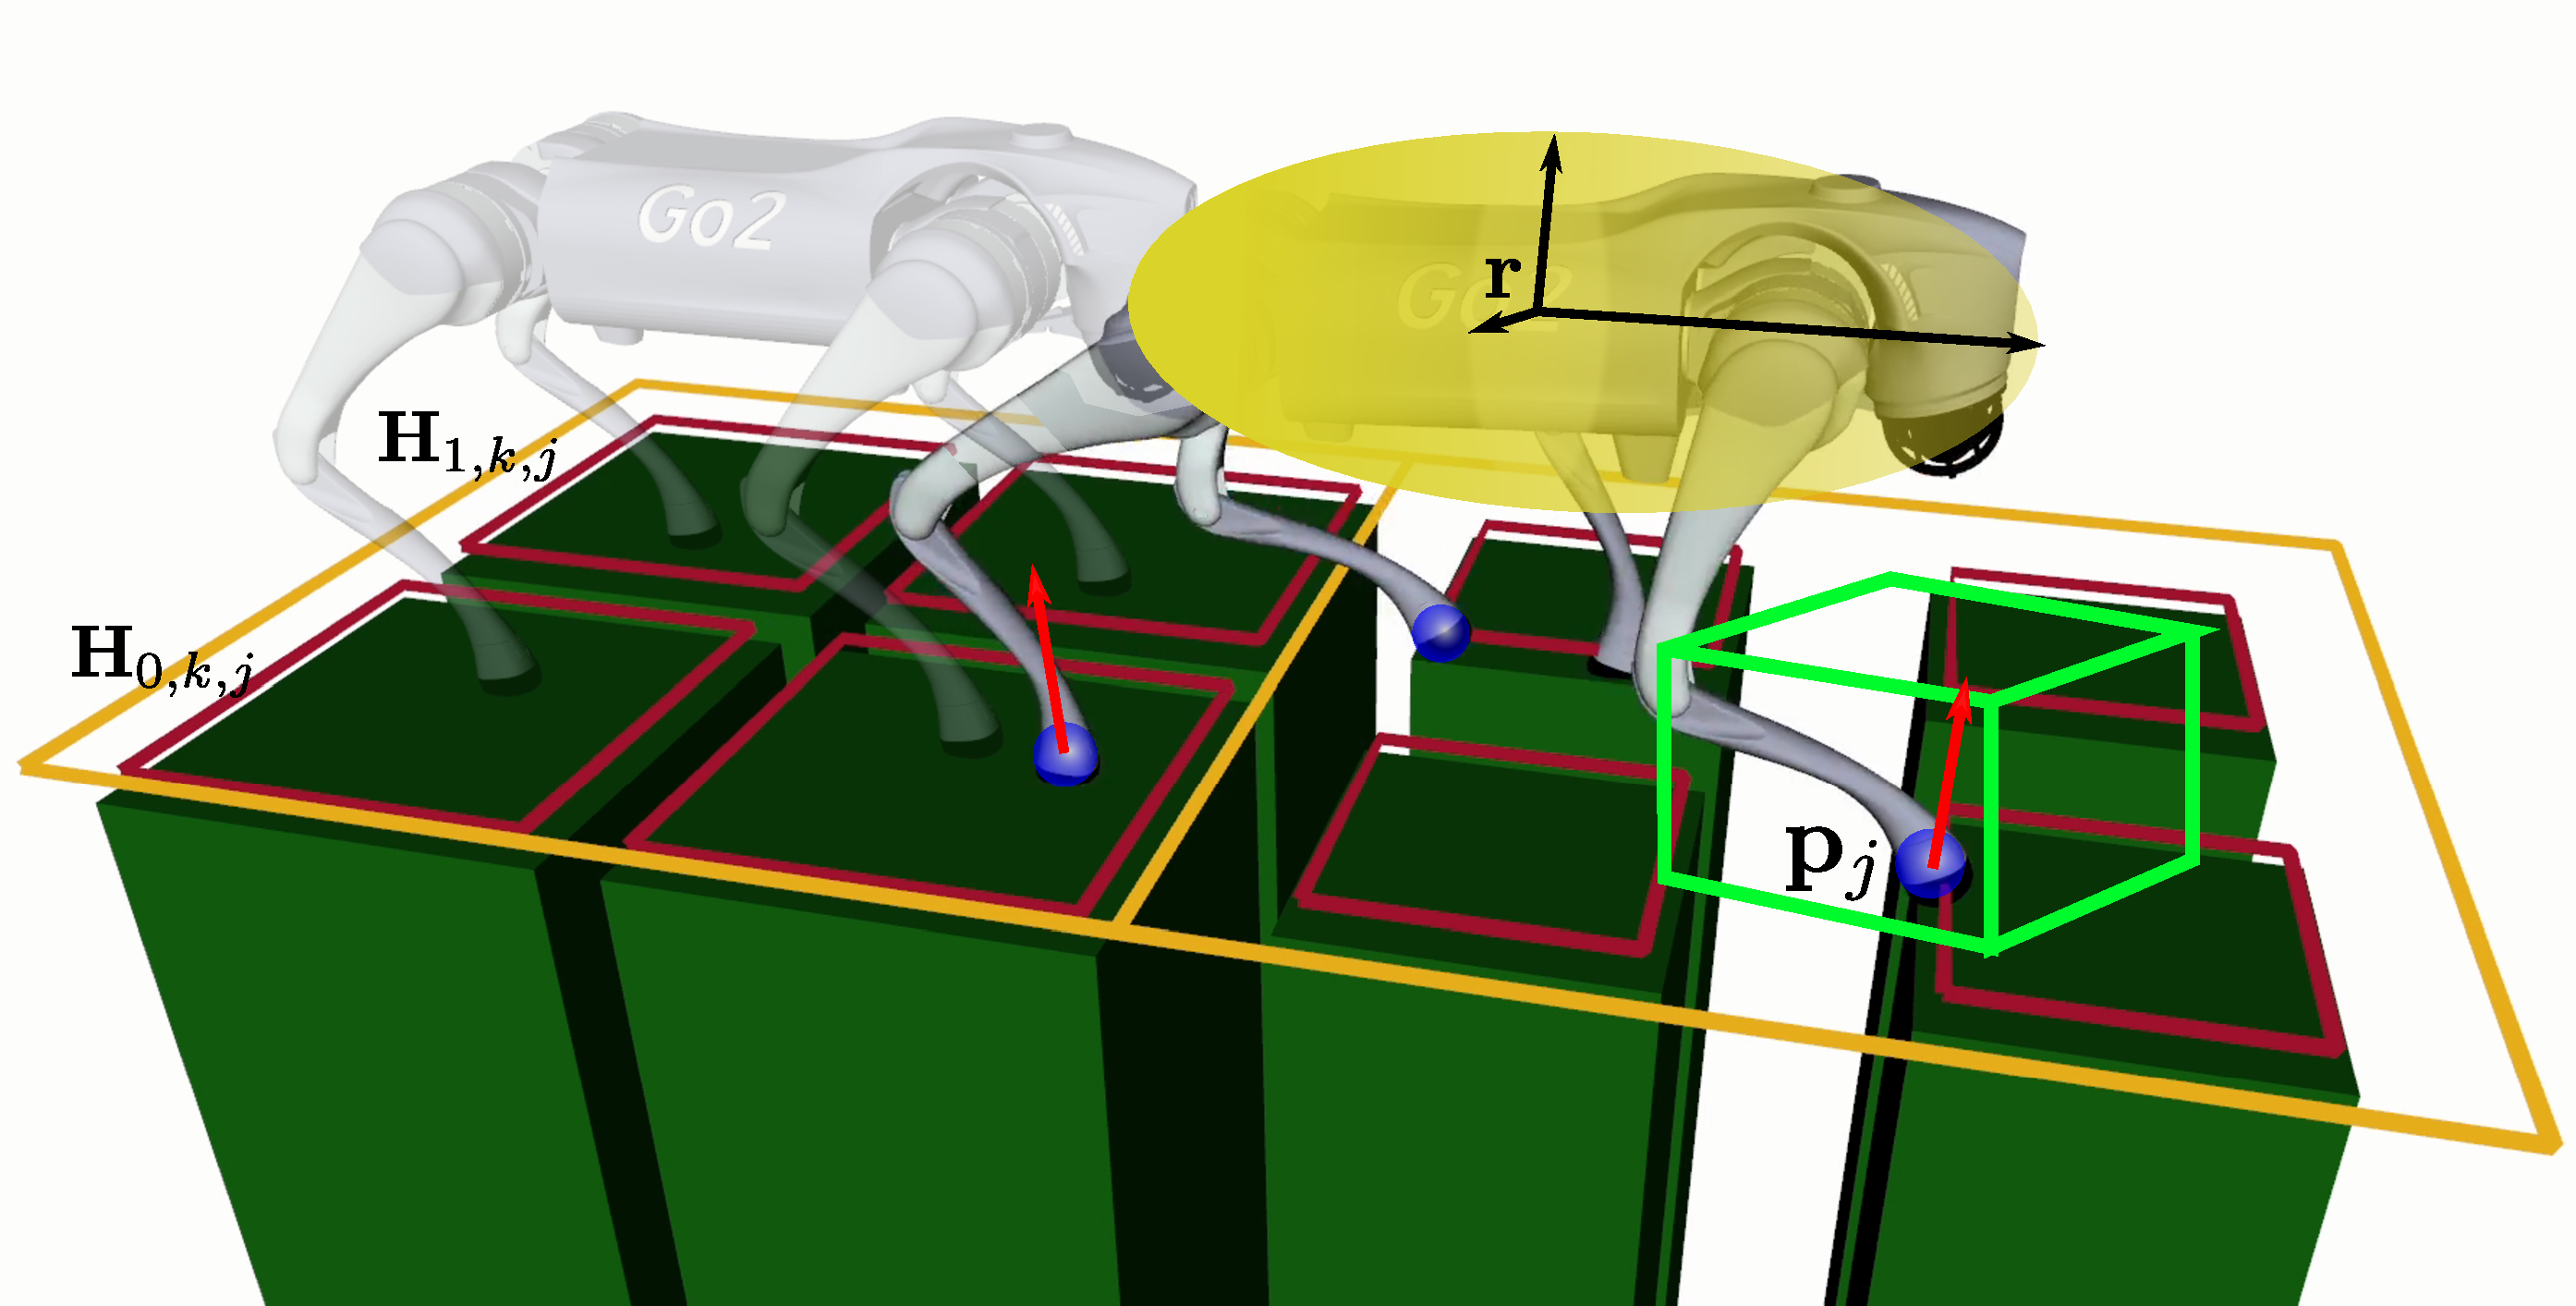
\includegraphics[width=0.9\linewidth]{mip_go2.pdf}
    \caption{Demonstration of decision variables and polygons when solving MICP for skill $a_0$ in Example~\ref{example:1} using a trotting locomotion gait.}
    \label{fig:mip_go2}
\end{figure}

The reference base position and angular trajectories are generated by linearly interpolating between the initial and final conditions. For scenarios with significant elevation changes, such as jumping onto higher terrain, an additional middle keyframe is introduced for the pitch angle to calculate the slope angle between the initial and final poses. The final reference pitch trajectory is then created by evenly interpolating between the initial, middle, and final poses. The reference EE trajectory relative to the base frame $^\mathcal{B} \v p_j^{\text{ref}}$ remains constant and moves in sync with the reference base trajectory. Given a specific locomotion gait, we first introduce the gait-fixed MICP formulation:

\subsubsection{Continuous Decision Variables}
The continuous decision variables $\vg \phi$ include base position $\v r$, velocity $\dot{\v r}$, acceleration $\ddot{\v r}$, orientation $\vg \theta$ parameterized by Euler angle and its first and second-order derivatives $\dot{\vg \theta},\ddot{\vg \theta}$, individual end-effector (EE) position $\v p_j$, velocity $\dot{\v p}_j$, and acceleration $\ddot{\v p}_j$, and individual contact force $\v f_j$ for the foot $j$ with $j\in\range{n_f}$, where $n_f=4$ denotes the index of feet. The compact form can be expressed as:
\begin{equation}
    \vg \phi = [\v r^\top, \dot{\v r}^\top, \ddot{\v r}^\top, \vg \theta^\top, \dot{\vg \theta}^\top, \ddot{\vg \theta}^\top, \v p_j^\top, \dot{\v p}_j^\top, \ddot{\v p}_j^\top, \v f_j^\top]^\top
\end{equation}

\subsubsection{System Dynamics}
We encode the system dynamics as a simplified single rigid body in Eq.~(\ref{eq:dynamics}),
using a double integrator to replace the original Euler equation to keep the dynamics constraint convex. The whole system is discretized through Backward Euler integration with $\Delta t$ between each time step.
\begin{equation}
        \label{eq:dynamics}
        \begin{bmatrix} \v r[i+1]\\\
        \dot{\v r}[i+1]\\\
        m \ddot{\v r}[i]\\\
        \vg \theta[i+1]\\
        \dot{\vg \theta}[i+1]
        \end{bmatrix}= \begin{bmatrix}
        \v r[i] + \Delta t \cdot \dot{\v r}[i+1]\\
        \dot {\v r}[i] + \Delta t \cdot \ddot{\v r}[i+1]\\
        \sum\nolimits_{j} \v f_j[i] + m \v g \\
	    % \sum\nolimits_j (\v{p}_j[i] - \v r[i]) \times \v f_j[i] \\
            \vg \theta[i] + \Delta t \cdot \dot{\vg \theta}[i+1]\\
            \dot{\vg \theta}[i] + \Delta t \cdot \ddot{\vg \theta}[i+1]
	    \end{bmatrix}
\end{equation}
where $m$ is the robot mass and $g$ is the gravity term.

\revised{We note that the rotational dynamics adopted in Eq.~(\ref{eq:dynamics}) are intentionally simplified: the rotational equation of motion is replaced by a double integrator on the Euler angles, which keeps the constraint convex but \textit{neglects the true angular-momentum dynamics.} This makes the formulation tractable for online deployment, but it limits applicability to highly dynamic motions such as flips or aggressive yaw maneuvers at high speeds.
%, or platforms where angular-momentum management is critical (e.g., humanoids).
Future work will explore convex relaxations of the full angular-momentum dynamics to expand the range of feasible motions while maintaining online tractability.}

\subsubsection{Cost Function}
The cost function consists of tracking costs and regularization terms governed by diagonal matrices $\v Q$ and $\v R$. 
\begin{equation}
    \v C = \delta \vg \phi_Q[i]^T\mathbf{Q}\hspace{2pt}\delta \vg \phi_Q[i] + \vg \phi_R[i]^{T}\mathbf{R}\vg \phi_R[i]
\end{equation}
where $\delta \vg \phi_Q$ and $\vg \phi_R$ are defined as:
\begin{equation}
    \delta \vg \phi_Q = \begin{bmatrix}
        \v r - \v r_{\text{ref}}\\
        \vg \theta - \vg \theta_{\text{ref}}\\
        \v p_j - \v p_{j}^{\text{ref}}
    \end{bmatrix}, \vg \phi_R = \begin{bmatrix}
        \ddot{\v r}\\
        \ddot{\vg \theta}\\
        \ddot{\v p}_j\\
        \v f_j
    \end{bmatrix}
\end{equation}

Tracking costs include deviation from the desired base and foot EE trajectories. The regularization term includes minimizing the base acceleration, Euler angle acceleration, EE acceleration, and contact forces to encourage motion smoothness. The weights for the tracking terms are defined in Table~\ref{tab:cost_weights}.

% \qm{plz also explain $N, n_f, n_s,$ and $R$}

% \subsubsection{Collision Avoidance}

\subsubsection{Safe Region Constraint}
To incorporate safe region constraints for selecting proper footholds, we introduce binary variables $\v H_{r,k,j}$, with $r$, $k$, and $j$ expressing the $r^{\rm th}$ convex region, $k^{\rm th}$ footstep, and $j^{\rm th}$ foot and $r\in\range{R}, k\in\range{n_s}$. One footstep is defined as a full swing phase for a foot. We use $n_s$ and $R$ to represent the number of footsteps specified by the gait configuration and the number of convex terrain polygons to be considered. For example,  Fig.~\ref{fig:mip_go2} shows a case with eight polygons.
Eqs.~(\ref{eq:safe_region}) - (\ref{eq:safe_region_eq}) restrict
the robot's EE to stay within one of the convex polygons when the corresponding binary variable $\v H_{r,k,j}$ is True. 
Each polygon is parameterized by an inequality constraint ($\v A_r$ and $\v b_r$) that defines multiple half-spaces, along with an equality constraint ($\v A_{\text{eq},r}$ and $\v b_{\text{eq},r}$) that ensures the foothold position lies on a 3D plane.
We use $\mathcal{C}_{k,j}$ to denote the set of time steps indicating stance after the $k^{\rm th}$ footstep for the $j^{\rm th}$ foot and the safe region constraint only applies to the first stance time step represented as $\mathcal{C}_{k,j}[0]$. Note that, during the offline phase, the terrain polygons are homogeneous and predefined.
\begin{align}
\nonumber
&\forall r \in [R], k \in [n_s], j \in [n_f]\\
    \label{eq:safe_region} &\v H_{r,k,j} \Rightarrow \v A_r \v p_j[i] \leq \v b_r, \forall i \in \mathcal{C}_{k,j}[0]
        \\\label{eq:safe_region_eq} & \hspace{1.5cm} \v A_{\text{eq},r} \v p_j[i] = \v b_{\text{eq},r}, \forall i \in \mathcal{C}_{k,j}[0]
        \\\label{eq:sum_contact_binary} &\sum_{r=0}^{R-1}\v H_{r,k,j} = 1
        \\&\v H_{r,k,j} \in \{0, 1\}
\end{align}

\subsubsection{Frictional and Contact Constraints}
Frictional constraints are defined in Eqs.~(\ref{eq:force_non_zero}) - (\ref{eq:force_friction_cone}), with $\v n_r$ and $\mathcal{F}_r$ as the normal vector and friction cone of the $r^{\rm th}$ convex region corresponding to the x and y dimensions of the EE position $\v p^{xy}_j$. Contact constraints in Eqs.~(\ref{eq:ee_velocity_zero}) - (\ref{eq:force_zero}) forces the EE velocity to be zero during stance phase and the contact force to be zero during the non-contact phase. $\mathcal{C}_{j}$ represents the set of all time steps indicating stance for the $j^{\rm th}$ foot.
\begin{align}
    \nonumber &\forall r \in [R], k \in [n_s], j \in [n_f]\\\label{eq:force_non_zero}
    &\v H_{r,k,j} \ \  \Rightarrow \ \ \v f_j[i] \cdot \v n_r(\v p_j^{xy}[i]) \ge 0, \ \forall i \in \mathcal{C}_{k,j}\\
    \label{eq:force_friction_cone}
        & \hspace{1.95cm} \v f_j[i] \in \mathcal{F}_r(\mu, \v n_r, \v p_j^{xy}[i]), \ \forall i \in \mathcal{C}_{k,j}
         \\\label{eq:ee_velocity_zero}
            &\dot{\v p}_j[i]=0, \ \forall i \in \mathcal{C}_j
        \\\label{eq:force_zero}
         &\v f_j[i] = 0, \ \forall i \notin \mathcal{C}_j
\end{align}
%
where $\mu$ denotes the friction coefficient.

\subsubsection{Actuation Constraint}
Since the joint angles are omitted in the single rigid body model, we use a fixed Jacobian $\v J_j(\v q_j^{\text{ref}})$ at a nominal joint pose $\v q_j^{\text{ref}}$ for each leg to approximately consider the torque limit constraint in Eq.~(\ref{eq:max_torque}). In addition, since the translational and angular motions are decoupled, another actuation constraint on the angular acceleration is also added in Eq.~(\ref{eq:max_acc}).
\begin{align}
\nonumber & \forall i \in [N], j \in [n_f] \\
    \label{eq:max_torque}
& \v J_j(\v q_j^{\text{ref}})^{\top} \v f_j[i] \leq \vg \tau_{\rm max}\\\label{eq:max_acc}
& \v I \ddot{\vg \theta}[i] \leq \vg \tau_{\rm max}^{\prime}
\end{align}
where $\vg \tau_{\rm max}$ is the joint torque limit, $\vg \tau_{\rm max}^{\prime}$ is the torque limit applied on the base, and $\v I$ is the moment of inertia for the approximated single rigid body.

\subsubsection{Kinematics Constraint}
Lastly, the kinematics constraint in Eq.~(\ref{eq:rom}) strictly limits the possible EE movements to assure safety.
% Fig.~\ref{fig:mip_a1} shows the essential decision variables optimized in \ref{ocp:mip_general}. 
Due to the convex nature of this MICP, we can determine the feasibility of a possible symbolic transition by checking if the optimal solution exists.
\begin{equation}
    \label{eq:rom}
    \v p_j[i] \in \mathcal{R}_j(^\mathcal{B} \v p_j^{\text{ref}}, \v r[i],\vg \theta_{\text{ref}}, \v p_j^{\text{max}}), \forall i \in [N], j \in [n_f]
\end{equation}
where $\mathcal{R}_j$ is defined as a 3D box constraint around a nominal foot EE position based on the base position and orientation, and constrained by a maximum deviation $\v p_j^{\text{max}}$. Note that the reference orientation $\vg \theta_{\text{ref}}$ is used to avoid nonlinear constraint keep the problem convex.

% \subsection{GR(1) Specifications given Robot Skills}\label{sec:spec_gen}
% \subsection{Task Specification Encoding}\label{sec:spec_gen}

% After acquiring a set of feasible robot skills, 
% we encode the skills into the specification $\spec$ 
% as part of the environment safety assumptions $\envsafety$ 
% and system safety guarantees $\syssafety$.
% %
% % We divide the safety assumptions $\envsafety$ into mutable assumptions $\envsafetynothard$,
% % which describe the postconditions of the skills,
% % and hard assumptions $\envsafetyhard$ that cannot be modified, 
% % i.e.
% % $\envsafety = \envsafetynothard \land \envsafetyhard$.
% % Similarly, we divide the safety guarantees $\syssafety$ into mutable guarantees $\syssafetynothard$,
% % which represent the preconditions of the skills,
% % and hard guarantees $\syssafetyhard$ that cannot be modified
% % ($\syssafety = \syssafetynothard \land \syssafetyhard$).
% %
% % To translate from states to formulas, 
% We define a function $\formplain$ that takes as input
% two subsets $\statevar, \statevar' \subseteq \ap$,
% where $\statevar \subseteq \statevar'$,
% and generates a Boolean formula
% $\form{\statevar'}{\statevar} \coloneqq \bigwedge_{\var\in\statevar}\var \land \bigwedge_{\var \in \statevar'\setminus\statevar} \neg\var$.
% For any subset $\statevar \subseteq \ap$,
% we use $\bigcirc\statevar$ to denote the set $\{\bigcirc \pi \mid \pi \in \statevar\}$.

% % We encode the postconditions of the skills into the environment safety assumptions $\envsafety$ of the specification $\spec$.



% % each skill $\texttt{skill} \in \mathcal{A}$ comes with a precondition $\sum_{\texttt{skill}}^{\rm{pre}} \in 2^{\mathcal{I}_G}$ and a postcondition $\sum_{\texttt{skill}}^{\rm{post}} \in 2^{\mathcal{I}_G}$ similar to \citep{pacheck2022physically}. In Fig.~\ref{fig:preliminary_nine_squares}(b) and (c), it shows a skill $\texttt{skill0}$ with precondition $\sum_{\texttt{skill0}}^{\rm{pre}} = \{(x=1,y=2,\rm cT = \rm Flat, \rm rT = \rm High)\}$ and postcondition $\sum_{\texttt{skill0}}^{\rm{post}} = \{(x=2,y=2)\}$. The skills are encoded in the GR(1) formula as part of $\phi^\textrm{t}_\textrm{e}$ and $\phi^\textrm{t}_\textrm{s}$, 
% % which can be further divided into $\phi^{\textrm{t}}_{\textrm{e}} = \phi^{\textrm{t, mutable}}_{\textrm{e}} \wedge \phi^{\textrm{t, hard}}_{\textrm{e}}$ and $\phi^{\textrm{t}}_{\textrm{s}} = \phi^{\textrm{t, mutable}}_{\textrm{s}} \wedge \phi^{\textrm{t, hard}}_{\textrm{s}}$. $\phi^{\textrm{t, mutable}}_{\textrm{e}}$ and $\phi^{\textrm{t, mutable}}_{\textrm{s}}$ capture the postconditions and preconditions that the repair process might modify, respectively. $\phi^{\textrm{t, hard}}_{\textrm{e}}$ and $\phi^{\textrm{t, hard}}_{\textrm{s}}$ encode the hard constraints specified by the user remain unchanged and always hold.   

% % \subsubsection{Postconditions}
% The skill assumptions $\envsafetynothard$ encode the postconditions of the skills. 
% % As shown in Eq.~\ref{eq:env_trans}, 
% The assumptions ensure that after the skill execution, 
% at least one postcondition of the skill must hold:
% % s in the next timestep:

% \begin{equation}\label{eq:env_trans}
% \begin{aligned}
%     \envsafetynothard \coloneqq \bigwedge_{\skill \in \mathcal{O}} \big( \skill 
%     % \land 
%     % \form{\inpcen\cup\inpterrain}{\skillpre} \\ 
%     \to
%     \bigvee_{\statevar\in\skillpost} \form{\bigcirc\inpcen}{\bigcirc\statevar} \big)
%     % \bigvee_{\sigma_\textrm{pre} \in \sum_{\texttt{skill}}^\textrm{pre}} \varphi_{\sigma_{\textrm{pre}}}) \rightarrow \\
%     % &\bigcirc \bigvee_{\sigma_\textrm{post} \in \sum_{\texttt{skill}}^\textrm{post}} \varphi_{\sigma_\textrm{post}}\bigg)
% \end{aligned}
% \end{equation}
% %
% In Example~\ref{fig:preliminary_nine_squares},
% % $\skillprecustom{\skillcustom{0}}$,
% the postcondition of skill $\skillcustom{0}$
% is defined as:
% % encoded asin Eq.~\ref{eq:skill_0_post}:
% % Therefore, as an example, the postcondition specification for $\texttt{skill0}$ is defined as:
% \begin{equation}\label{eq:skill_0_post}
% \begin{aligned}
%      \square (\skillcustom{0} 
%      % \land x_1 \land y_1 \land \tvar{x_1}{y_0} \land \tvar{x_1}{y_1} \land \tvar{x_1}{y_2}
%      % \land \bigwedge_{\var\in\inpcen\cup\inpterrain\setminus\skillprecustom{\skillcustom{0}}} \neg \var \\
%     \to &\bigcirc x_0 \land \bigcirc y_1 \land \neg \dots)
%     % &\neg \bigcirc x_1 \land 
%     % \neg \bigcirc x_2 \land 
%     % \neg \bigcirc y_0 \land 
%     % \neg \bigcirc y_2 \big)
%      % \bigwedge_{\var\in\inpcen\setminus\skillpostcustom{\skillcustom{0}}} \neg \bigcirc \var \big)
%      % x=1 \wedge y=2 \wedge \rm cT = \rm Flat \wedge \rm rT = \rm High \big) \rightarrow \\
%      % &\bigcirc \big(x=2 \wedge y=2 \big) \big)
% \end{aligned}
% \end{equation}
% where we omit the centroidal inputs that are False.

% % \subsubsection{Preconditions}
% The skill guarantees $\syssafetynothard$ encode the preconditions of the skills.
% The guarantees impose restrictions on when a skill can be executed.
% % As shown in Eq.~\ref{eq:sys_trans},
% The guarantees only allow the robot to execute a skill 
% if one of the skill's preconditions holds:
% % The preconditions encode constraints in $\varphi_{\textrm s}^{\textrm{t}, \textrm{mutable}}$. It restricts the conditions that a specific skill can be chosen. Therefore, it allows the overall system to choose a skill only when a precondition is satisfied, but does not require the system to do so. 

% \begin{equation}\label{eq:sys_trans}
% \begin{aligned}
%     \syssafetynothard \coloneqq 
%     \bigwedge_{\skill \in \mathcal{O}} \bigg(
%     \neg \big(
%     \bigvee_{\statevar\in\skillprecustom{\skill}}
%     \form{\bigcirc\inpcen\cup\bigcirc\inpterrain}{\bigcirc\statevar}
%     \big)
%     % \\
%     % \form{\bigcirc(\inpcen\cup\inpterrain)}{\bigcirc\skillprecustom{\skill}}\\
%     \to \neg \bigcirc \skill
%     \bigg)
%     % \\
%     % \varphi_{\textrm s}^{\textrm{t}, \textrm{mutable}} = \bigwedge_{\pi_{\texttt{skill}} \in \mathcal{O}} \bigg( & \neg (\bigcirc \bigvee_{\sigma_\textrm{pre} \in \sum_{\texttt{skill}}^\textrm{pre}} \varphi_{\sigma_{\textrm{pre}}}) \rightarrow 
%     % &\neg \bigcirc \pi_{\texttt{skill}}\bigg)
% \end{aligned}
% \end{equation}
% %
% In Example~\ref{example:1}, the precondition of skill $\skillcustom{0}$ is defined as:
% \begin{equation}
% \begin{aligned}
%      \square \big( \neg 
%      (
%      \bigcirc x_1 \land 
%      \bigcirc y_1 \land 
%      \bigcirc \tvar{x_1}{y_0} \land 
%      \bigcirc \tvar{x_1}{y_1} \land 
%      \bigcirc \tvar{x_1}{y_2}\land \\
%      \neg \dots)
%      % \neg \bigcirc x_0 \land
%      % \neg \bigcirc x_2 \land
%      % \neg \bigcirc y_0 \land
%      % \neg \bigcirc y_2 \land \\
%      % \bigwedge_{i\in\{0,2\}, j\in\{0,1,2\}}
%      % \neg \bigcirc \tvar{x_i}{y_j}\big)
%      % \bigwedge_{\var\in\inpcen\cup\inpterrain\setminus\skillprecustom{\skillcustom{0}}} \neg \bigcirc \var
%      % \big)
%      % \\
%      \to \neg \bigcirc \skillcustom{0} \big)
%      % \\
%      % (\bigcirc (x=1 \wedge y=2 \wedge \rm cT = \rm Flat \wedge \rm rT = \rm High)) \rightarrow \\
%      % \neg \bigcirc \pi_\texttt{skill0}\big)
% \end{aligned}
% \end{equation}
% where we omit the centroidal and terrain inputs that are False.
% % include the keyframe transition action $\mathcal{K}$ and gait primitives $\mathcal{G}$. We further divide $\mathcal{G}$ into $\mathcal{G} = \{\rm{gaitType}, \rm{gaitSpeed}\}$. We incorporate extra input propositions $\mathcal{E}$ to represent the terrain information, which shows up in the preconditions as well.
% % \subsubsection{Hard Constraints}\label{sec:hard_constraints}

% The hard constraints ($\envsafetyhard$, $\syssafetyhard$) are constraints that a repair cannot modify 
% (see Sec.~\ref{sec:symbolic_repair}).
% To strictly guarantee $\syssafetyhard$,
% we only allow the robot to execute one skill at a time:
%     $\square\big(\neg (\bigcirc\skill \land \bigcirc\skill')\big)$, for any two different skills $\skill, \skill' \in \out$. Given that, 
%     %such that $\skill \neq \skill'$.
% we encode the following hard assumptions $\envsafetyhard$:
% % as hard constraints in $\envsafetyhard$ and $\syssafetyhard$:
% % The hard assumptions $\envsafetyhard$ states that
% \begin{enumerate}[label=\arabic*),ref=\arabic*]
%     \item The uncontrollable terrain and request inputs 
%     % $\inpterrain \cup \inprequest$
%     % which include the terrain and request inputs ($\inpuser = \inpterrain\cup\inprequest$), 
%     cannot change during execution:
%     % $\forall \var \in \inpuser$,
%     $\square (\var \leftrightarrow \bigcirc \var)$,
%     $\forall \var \in \inpterrain \cup \inprequest$.
%     \item The centroidal inputs $\inpcen$ remain unchanged if no skill is executed: 
%     $\square\big(\bigwedge_{\skill\in\out} \neg \skill \to \bigwedge_{\var\in\inpcen} (\var \leftrightarrow \bigcirc \var)\big)$.
%     \item \label{assumption:poss_terrain}
%     The terrain state must come from the set of possible terrain states $\inpstateterrainposs \subseteq 2^{\inpterrain}$ provided by the user:
%     $\envterrain \coloneqq \square (
%     \bigvee_{\statevar\in\inpstateterrainposs}
%     \form{\inpterrain}{\statevar}
%     )$.
% \end{enumerate}
\begin{table}[t]
\centering
    \caption{Tracking Cost Weights}
    \setlength{\tabcolsep}{4pt}
     \begin{tabular}{ll}
         \hline
         \textbf{Cost Term} & \textbf{Weights}\\\hline
         $\v r - \v r_{\text{ref}}$ & (1000.0, 1000.0, 1000.0)\\
         $\vg \theta - \vg \theta_{\text{ref}}$ & (1000.0, 1000.0, 1000.0)\\
         $\v p_j - \v p_{j}^{\text{ref}}$ & (1000.0, 1000.0, 1000.0)\\
         $\ddot{\v r}$ & (10.0, 10.0, 10.0)\\
         $\ddot{\vg \theta}$ & (10.0, 10.0, 10.0)\\
         $\ddot{\v p}_j$ & (0.5, 0.5, 0.5)\\
         $\v f_j$ & (0.1, 0.1, 0.1)\\
         \hline
    \end{tabular}
    \label{tab:cost_weights}
\end{table}
\subsection{Task Specification Encoding}\label{sec:spec_gen}

% After acquiring a set of feasible robot skills, 
% we encode the skills into the specification $\spec$ 
% as part of the environment safety assumptions $\envsafety$ 
% and system safety guarantees $\syssafety$.

% The skill assumptions $\envsafetynothard$ encode the postconditions of the skills. 
% The assumptions ensure that after the skill execution when the precondition holds, 
% at least one postcondition of the skill must hold:

After identifying a set of feasible robot skills, we encode them into the specification $\spec$ as part of the environment safety assumptions $\envsafety$ and the system safety guarantees $\syssafety$. \revised{Each skill is associated with a user-defined precondition set $\skillpre \subseteq 2^{\inpcen \cup \inpterrain}$ and postcondition set $\skillpost \subseteq 2^{\inpcen}$, expressed over the robot and terrain inputs introduced in Sec.~\ref{sec:preliminaries_abstraction}. The encoding rules below map these sets into the GR(1) components $\envsafetynothard$ and $\syssafetynothard$ deterministically.}

The environment-side skill assumptions $\envsafetynothard$ capture the postconditions of each skill. These assumptions enforce that whenever a skill’s precondition holds and the skill is executed, at least one of its associated postconditions must also hold:
\begin{equation}
\begin{aligned}
    \envsafetynothard \coloneqq \bigwedge_{\skill \in \mathcal{O}} 
\square
% \big
((\skill 
    \land
    \bigvee_{\statevar\in\skillprecustom{\skill}}
    \bigwedge_{\var\in \inpcen \cup \inpterrain} \var=\statevar(\var))\\
    % \form{\inpcen\cup\inpterrain}{\skillpre} \\ 
    \to
    \bigvee_{\statevar\in\skillpost} 
    \bigwedge_{\var \in \inpcen}
    % \form{\bigcirc\inpcen}
    {\bigcirc (\var=\statevar(\var))} 
    % \big
    )
\end{aligned}
\end{equation}
% $\envsafetynothard \coloneqq \bigwedge_{\skill \in \mathcal{O}} 
% \square
% % \big
% ( \skill 
%     % \land 
%     % \form{\inpcen\cup\inpterrain}{\skillpre} \\ 
%     \to
%     \bigvee_{\statevar\in\skillpost} 
%     \bigwedge_{\var \in \inpcen}
%     % \form{\bigcirc\inpcen}
%     {\bigcirc (\var=\statevar(\var))} 
%     % \big
%     )
% $.
% s in the next timestep:
% \begin{equation*}\label{eq:env_trans}
% \begin{aligned}
%     \envsafetynothard \coloneqq \bigwedge_{\skill \in \mathcal{O}} \big( \skill 
%     % \land 
%     % \form{\inpcen\cup\inpterrain}{\skillpre} \\ 
%     \to
%     \bigvee_{\statevar\in\skillpost} \form{\bigcirc\inpcen}{\bigcirc\statevar} \big)
%     % \bigvee_{\sigma_\textrm{pre} \in \sum_{\texttt{skill}}^\textrm{pre}} \varphi_{\sigma_{\textrm{pre}}}) \rightarrow \\
%     % &\bigcirc \bigvee_{\sigma_\textrm{post} \in \sum_{\texttt{skill}}^\textrm{post}} \varphi_{\sigma_\textrm{post}}\bigg)
% \end{aligned}
% \end{equation*}
%
In Example~\ref{example:1},
% $\skillprecustom{\skillcustom{0}}$,
the postcondition of skill $\skillcustom{0}$
is defined as
\begin{equation}
\begin{aligned}
    \square (\skillcustom{0} 
     \land \var_{x_1} \land \var_{y_1} \land \tvar{x_1}{y_0} = 1 \land \tvar{x_1}{y_1} = 1 \land \tvar{x_1}{y_2} = 1 \land \dots \\
     % \land \bigwedge_{\var\in\inpcen\cup\inpterrain\setminus\skillprecustom{\skillcustom{0}}} \neg \var \\
    \to \bigcirc \var_{x_0} \land \bigcirc \var_{y_1} \land \neg \dots)
\end{aligned}
\end{equation}
% $
% \square (\skillcustom{0} 
%      % \land x_1 \land y_1 \land \tvar{x_1}{y_0} \land \tvar{x_1}{y_1} \land \tvar{x_1}{y_2}
%      % \land \bigwedge_{\var\in\inpcen\cup\inpterrain\setminus\skillprecustom{\skillcustom{0}}} \neg \var \\
%     \to \bigcirc \var_{x_0} \land \bigcirc \var_{y_1} \land \neg \dots)
% $.
% encoded asin Eq.~\ref{eq:skill_0_post}:
% Therefore, as an example, the postcondition specification for $\texttt{skill0}$ is defined as:
% \begin{equation*}\label{eq:skill_0_post}
% \begin{aligned}
%      \square (\skillcustom{0} 
%      % \land x_1 \land y_1 \land \tvar{x_1}{y_0} \land \tvar{x_1}{y_1} \land \tvar{x_1}{y_2}
%      % \land \bigwedge_{\var\in\inpcen\cup\inpterrain\setminus\skillprecustom{\skillcustom{0}}} \neg \var \\
%     \to &\bigcirc x_0 \land \bigcirc y_1 \land \neg \dots)
%     % &\neg \bigcirc x_1 \land 
%     % \neg \bigcirc x_2 \land 
%     % \neg \bigcirc y_0 \land 
%     % \neg \bigcirc y_2 \big)
%      % \bigwedge_{\var\in\inpcen\setminus\skillpostcustom{\skillcustom{0}}} \neg \bigcirc \var \big)
%      % x=1 \wedge y=2 \wedge \rm cT = \rm Flat \wedge \rm rT = \rm High \big) \rightarrow \\
%      % &\bigcirc \big(x=2 \wedge y=2 \big) \big)
% \end{aligned}
% \end{equation*}
% We omit the robot inputs that are $\false$ for space.
% that are False for space.

% \subsubsection{Preconditions}
% The skill guarantees $\syssafetynothard$ encodes the preconditions of the skills.
% The guarantees impose restrictions on when a skill can be executed.
% The guarantees only allow the robot to execute a skill 
% if one of the skill's preconditions holds:
The system-side skill guarantees $\syssafetynothard$ encode the preconditions associated with each skill. These guarantees restrict when a skill may be executed by the robot. Specifically, a skill is permitted to run only if at least one of its preconditions is satisfied:
% The preconditions encode constraints in $\varphi_{\textrm s}^{\textrm{t}, \textrm{mutable}}$. It restricts the conditions that a specific skill can be chosen. Therefore, it allows the overall system to choose a skill only when a precondition is satisfied, but does not require the system to do so. 
\begin{equation}
\begin{aligned}
    \syssafetynothard \coloneqq 
    \bigwedge_{\skill \in \mathcal{O}} 
    \square (
    \neg (
    \bigvee_{\statevar\in\skillprecustom{\skill}}
    \bigwedge_{\var\in \inpcen \cup \inpterrain}
    % \form{\bigcirc\inpcen\cup\bigcirc\inpterrain}
    {\bigcirc(\var = \statevar(\var))}
    )
    \\
    % \form{\bigcirc(\inpcen\cup\inpterrain)}{\bigcirc\skillprecustom{\skill}}\\
    \to \neg \bigcirc \skill)
\end{aligned}
\end{equation}
\revised{The disjunction $\bigvee_{\statevar \in \skillpre}$ in the equation above is taken over precondition pairs in $\skillpre$: a skill becomes eligible to execute when the conjunction of input assignments specified by at least one full pair $(\inpstatecen, \inpstateterrain) \in \skillpre$ holds, rather than when only some individual atomic propositions within a pair hold.}
% $
% \syssafetynothard \coloneqq
%     \bigwedge_{\skill \in \mathcal{O}} 
%     \square (
%     \neg (
%     \bigvee_{\statevar\in\skillprecustom{\skill}}
%     \bigwedge_{\var\in \inpcen \cup \inpterrain}
%     % \form{\bigcirc\inpcen\cup\bigcirc\inpterrain}
%     {\bigcirc(\var = \statevar(\var))}
%     )
%     % \\
%     % \form{\bigcirc(\inpcen\cup\inpterrain)}{\bigcirc\skillprecustom{\skill}}\\
%     \to \neg \bigcirc \skill)
% $.
% \begin{equation*}\label{eq:sys_trans}
% \begin{aligned}
%     \syssafetynothard \coloneqq 
%     \bigwedge_{\skill \in \mathcal{O}} \bigg(
%     \neg \big(
%     \bigvee_{\statevar\in\skillprecustom{\skill}}
%     \form{\bigcirc\inpcen\cup\bigcirc\inpterrain}{\bigcirc\statevar}
%     \big)
%     % \\
%     % \form{\bigcirc(\inpcen\cup\inpterrain)}{\bigcirc\skillprecustom{\skill}}\\
%     \to \neg \bigcirc \skill
%     \bigg)
%     % \\
%     % \varphi_{\textrm s}^{\textrm{t}, \textrm{mutable}} = \bigwedge_{\pi_{\texttt{skill}} \in \mathcal{O}} \bigg( & \neg (\bigcirc \bigvee_{\sigma_\textrm{pre} \in \sum_{\texttt{skill}}^\textrm{pre}} \varphi_{\sigma_{\textrm{pre}}}) \rightarrow 
%     % &\neg \bigcirc \pi_{\texttt{skill}}\bigg)
% \end{aligned}
% \end{equation*}
%
In Example~\ref{example:1}, the precondition of skill $\skillcustom{0}$ is defined as
\begin{equation}
\begin{aligned}
\square \big( \neg 
     (
     \bigcirc \var_{x_1} \land 
     \bigcirc \var_{y_1} \land
     \bigcirc \tvar{x_1}{y_0}=1 \land 
     \bigcirc \tvar{x_1}{y_1}=1 \land 
     \\
     \bigcirc \tvar{x_1}{y_2}=1 \land 
     \dots)
     % \neg \bigcirc x_0 \land
     % \neg \bigcirc x_2 \land
     % \neg \bigcirc y_0 \land
     % \neg \bigcirc y_2 \land \\
     % \bigwedge_{i\in\{0,2\}, j\in\{0,1,2\}}
     % \neg \bigcirc \tvar{x_i}{y_j}\big)
     % \bigwedge_{\var\in\inpcen\cup\inpterrain\setminus\skillprecustom{\skillcustom{0}}} \neg \bigcirc \var
     % \big)
     \to \neg \bigcirc \skillcustom{0} \big)
\end{aligned}
\end{equation}
% \begin{equation*}
% \begin{aligned}
%      \square \big( \neg 
%      (
%      \bigcirc x_1 \land 
%      \bigcirc y_1 \land 
%      \bigcirc \tvar{x_1}{y_0} \land 
%      \bigcirc \tvar{x_1}{y_1} \land 
%      \bigcirc \tvar{x_1}{y_2}\land 
%      \dots)
%      % \neg \bigcirc x_0 \land
%      % \neg \bigcirc x_2 \land
%      % \neg \bigcirc y_0 \land
%      % \neg \bigcirc y_2 \land \\
%      % \bigwedge_{i\in\{0,2\}, j\in\{0,1,2\}}
%      % \neg \bigcirc \tvar{x_i}{y_j}\big)
%      % \bigwedge_{\var\in\inpcen\cup\inpterrain\setminus\skillprecustom{\skillcustom{0}}} \neg \bigcirc \var
%      % \big)
%      % \\
%      \to \neg \bigcirc \skillcustom{0} \big)
%      % \\
%      % (\bigcirc (x=1 \wedge y=2 \wedge \rm cT = \rm Flat \wedge \rm rT = \rm High)) \rightarrow \\
%      % \neg \bigcirc \pi_\texttt{skill0}\big)
% \end{aligned}
% \end{equation*}
% We use
% Boolean propositions
% to represent
% % Note that 
% the integer terrain inputs.
% % is represented by a set of  
% We omit the robot inputs that are $\false$ and the terrain inputs whose values are $0$ 
% for space.
% include the keyframe transition action $\mathcal{K}$ and gait primitives $\mathcal{G}$. We further divide $\mathcal{G}$ into $\mathcal{G} = \{\rm{gaitType}, \rm{gaitSpeed}\}$. We incorporate extra input propositions $\mathcal{E}$ to represent the terrain information, which shows up in the preconditions as well.
% \subsubsection{Hard Constraints}\label{sec:hard_constraints}

The hard constraints $\envsafetyhard$ and $\syssafetyhard$ are constraints that a repair cannot modify 
(see Sec.~\ref{sec:manager_and_repair}).
Our system's hard constraints
$\syssafetyhard$
only allow the robot to execute one skill at a time:
    $\square\big(\neg (\bigcirc\skill \land \bigcirc\skill')\big)$, for any two different skills $\skill, \skill' \in \out$. 
%
Given that, 
    %such that $\skill \neq \skill'$.
we encode the following hard assumptions $\envsafetyhard$:
% as hard constraints in $\envsafetyhard$ and $\syssafetyhard$:
% The hard assumptions $\envsafetyhard$ states that
\begin{enumerate}[label=(\roman*),ref=\roman*]
    \item the uncontrollable terrain and request inputs 
    % $\inpterrain \cup \inprequest$
    % which include the terrain and request inputs ($\inpuser = \inpterrain\cup\inprequest$), 
    cannot change during execution:
    % $\forall \var \in \inpuser$,
    $\square (\var \leftrightarrow \bigcirc \var)$,
    $\forall \var \in \inpterrain \cup \inprequest$,
    and
    \item the robot inputs $\inpcen$ remain unchanged if no skill is executed: 
    $\square\big(\bigwedge_{\skill\in\out} \neg \skill \to \bigwedge_{\var\in\inpcen} (\var \leftrightarrow \bigcirc \var)\big)$.
    % \item \label{assumption:poss_terrain}
    % The terrain state must come from the set of possible terrain states $\inpstateterrainposs \subseteq 2^{\inpterrain}$ provided by the user:
    % $\envterrain \coloneqq \square (
    % \bigvee_{\statevar\in\inpstateterrainposs}
    % \form{\inpterrain}{\statevar}
    % )$.
\end{enumerate}

% Certain constraints also need to be incorporated as hard constraints. $\varphi_{\textrm e}^{\textrm{t}, \textrm{hard}}$ and $\varphi_{\textrm s}^{\textrm{t}, \textrm{hard}}$. For instance, specifications such as enforcing movements among adjacent grids are encoded as hard constraints. Other constraints such as the mutual exclusion of different skills are also added here. 

% For the nine-square example, we 

% Due to the space limit, we only highlight the specifications that build connections between the environment and the robot action. We construct the following specifications based on locomotion heuristics:

% Hard specifications. React to terrain abstraction. Mutual exclusion of each skill and each grounded state.



% \subsection{Offline Synthesis with Feasibility Check}
% Fig.~\ref{fig:combined_offline_online} illustrates the system overview for both offline synthesis and online execution. This section focuses on the offline synthesis process. Using prior knowledge provided by humans, we first define a set of motion primitives, such as a one-second trotting gait, and a set of potential terrains described at the symbolic level. Based on the abstracted robot and terrain states defined in Sec.\ref{sec:preliminaries_abstraction}, we iterate over the grid locations and solve the MICP to check if a solution exists when the desired goal is the adjacent grid. If a solution is found, the corresponding skill is added to the specification. Once the hard constraints and physically feasible skills are incorporated into the specification, we assess its realizability. If it is realizable, a strategy is generated for online execution. If not, an offline repair is introduced, as discussed in the next section.

% \subsection{Symbolic Repair}\label{sec:symbolic_repair}
% The specification $\spec$ generated in Sec.~\ref{sec:spec_gen} may be unrealizable
% if the physical feasibility checking in Sec.~\ref{sec:motion_primitive} does not generate enough skills for the robot to reach all goal locations over all possible terrain combinations.
% %
% To adress this issue, we leverage the ideas in~\citep{pacheck2022physically} 
% to
% generate
% new skill suggestions necessary for the robot to accomplish the task.
% %over all possible terrain environments.
% Different from~\citep{pacheck2022physically}, we assume that skills do not contain intermediate states,
% and the skill preconditions
% are over both the controllable centroidal inputs $\inpcen$ and uncontrollable terrain inputs $\inpterrain$, 
% while the postconditions remain to contain 
% controllable
% centroidal inputs $\inpcen$ only.

% For any subset $\statevar\subseteq \ap$, we say that $\statevar$ is a winning state
% if the robot can guarantee to satisfy the task from $\statevar$
% despite adversarial environment behaviors.
% The repair process systematically expands the set of winning states until
% it intersects with all liveness goals and contains all initial states.
% To this end, the repair alternatively modifies the preconditions and postconditions of existing skills.
% When modifying preconditions, the repair randomly selects a skill whose postcondition is winning, and modifies its precondition to a non-winning state, thus making the new precondition possible to win.
% When modifying postconditions, the repair randomly selects a skill whose preconditions and postconditions are both non-winning, and modifies its postcondition to a winning state, thus making the original precondition possible to win.
% %
% Fig~\ref{fig:preliminary_nine_squares}c illustrates the use of repair in Example~\ref{example:1}. 
% To create a skill that reaches the requested grid $(x_0, y_0)$, the
% repair selects the skill transition that moves the robot from the grid $(x_1, y_0)$ to $(x_2, y_0)$,
% and modifies the postcondition to reach $(x_0, y_0)$ instead. Finally, the suggested skills are sent to a gait reconfiguration module for feasibility checking. If any suggested skill is found infeasible, the symbolic transition is added as a hard constraint, and the repair process is repeated.

\subsection{High-level Manager and Symbolic Repair}\label{sec:manager_and_repair}
% The encoded specification $\spec$ has a large state space since it needs to encode the surrounding terrain states.
% Due to the exponential time complexity of the GR(1) synthesis algorithm in the size of the atomic propositions,
% it is impractical to synthesize a controller for $\spec$.
% \qm{probably can move above to intro}
%

% Similar to \citep{zhou2025physically}, we design a high-level manager
% to 
% efficiently synthesize controllers for
% the encoded specification
% under given sets of terrain and request states.
% The manager takes in 
% the specification $\spec$,
% a predefined set of terrain states 
% $\inpstatesterrainexprposs \subseteq \inpstatesterrain$,
% and
% a predefined set of request states 
% $\inpstatesrequestposs \subseteq \inpstatesrequest$.
% For every pair of integer terrain and request state 
% $(\inpstateterrain, \inpstaterequest) \in \inpstatesterrainexprposs \times \inpstatesrequestposs$,
% the manager 
% first translates
% the integer terrain state $\inpstateterrain: \inpterrain \to \range{n_t}$
% to its corresponding Boolean terrain state
% $\inpstateterrainbool: \inpterrainbool \to \{\true, \false\}$,
% using a set of Boolean propositions $\inpterrainbool$ to represent the integer terrain inputs $\inpterrain$,
% as done in~\citep{ehlers2016slugs}.
% We overload $\inpstateterrainbool$ and $\inpstaterequest$
% to represent the inputs that are $\true$
% in $\inpstateterrainbool$ and $\inpstaterequest$.
% The manager then
% generates a partial evaluation
% $\spec' \coloneqq \spec[\inpstateterrainbool \cup \inpstaterequest, \inpterrainbool \cup \inprequest \setminus \inpstateterrainbool \cup \inpstaterequest]$ (see Definition~\ref{def:partial_eval}).
% Next,
% we remove skills that cannot be executed in the local environment, i.e., their preconditions are evaluated to $\false$ under the partial evaluation.
% Since
% the inputs of $\spec'$ only include the robot inputs $\inpcen$
% and the outputs of $\spec'$ consist of fewer skills,
% we avoid the exponential blow-up of the synthesis algorithm in the size of the variables.
% Lastly,
% the manager synthesizes a strategy $\strategy_{\spec'}$ for each $\spec'$.

% The partial evaluation $\spec'$ can be unrealizable
% if the gait-fixed MICP-based 
% physical feasibility checking 
% in Sec.~\ref{sec:motion_primitive} 
% does not generate enough skills for the robot to reach the requested goal under the terrain state.
% To add more robot skills,
% we will leverage a gait-free MICP (formulated in Sec.~\ref{sec:gait_free_micp})
% which retains all continuous decision variables and constraints from the gait-fixed MICP 
% but modifies the contact state-dependent constraints 
% so that the contact sequence and timing are no longer fixed.
% Since
% such a gait-free MICP is 
% computationally expensive,
% we leverage a symbolic repair tool~\citep{pacheck2022physically}
% to 
% generate symbolic suggestions that 
% guide us to perform 
% necessary gait-free MICP only.
% Given an unrealizable $\spec'$,
% symbolic repair systematically
% modifies the pre- and postconditions of existing skills
% to suggest new skills that make $\spec'$ 
% realizable,
% if such skills exist and are physically feasible.
% Fig.~\ref{fig:preliminary_nine_squares}(c) illustrates the use of repair in Example~\ref{example:1}. 
% To create a skill that reaches the requested grid $(x_0, y_0)$,
% repair selects the skill transition that moves the robot from the grid $(x_1, y_0)$ to $(x_2, y_0)$,
% and modifies the postcondition to be $(x_0, y_0)$.
% Similar to \citep{zhou2025physically}, 
We design a high-level manager to efficiently synthesize controllers for encoded specifications under given sets of terrain and request states. The manager takes as input the specification $\spec$, a predefined collection of terrain states $\inpstatesterrainexprposs \subseteq \inpstatesterrain$, and a predefined set of request states $\inpstatesrequestposs \subseteq \inpstatesrequest$. For each pair $(\inpstateterrain, \inpstaterequest) \in \inpstatesterrainexprposs \times \inpstatesrequestposs$, the manager first converts the integer-valued terrain state $\inpstateterrain: \inpterrain \to \range{n_t}$ into a Boolean representation $\inpstateterrainbool: \inpterrainbool \to \{\true, \false\}$, following the approach in \citep{ehlers2016slugs}. We then overload $\inpstateterrainbool$ and $\inpstaterequest$ to denote the propositions that evaluate to $\true$. Using this, the manager generates a partial evaluation $\spec' \coloneqq \spec[\inpstateterrainbool \cup \inpstaterequest, \inpterrainbool \cup \inprequest \setminus \inpstateterrainbool \cup \inpstaterequest]$ (see Definition~\ref{def:partial_eval}). Skills whose preconditions are evaluated to $\false$ under the partial evaluation are discarded, which reduces the specification to robot inputs $\inpcen$ and a smaller skill set as outputs. This step prevents exponential growth of the synthesis procedure in the variable size. Finally, the manager synthesizes a strategy $\strategy_{\spec'}$ for each reduced specification.

If $\spec'$ is unrealizable, this indicates that gait-fixed MICP feasibility checks (Sec.~\ref{sec:motion_primitive}) failed to produce sufficient skills to reach the request under the given terrain. To address this, we rely on gait-free MICP (Sec.~\ref{sec:gait_free_micp}), which relaxes the fixed contact sequence and timing constraints while retaining the continuous dynamics. Since gait-free MICP is computationally demanding, we employ symbolic repair \citep{pacheck2022physically} to generate targeted symbolic suggestions that minimize unnecessary solves. Symbolic repair works by systematically modifying pre- and postconditions of existing skills to propose new candidates. These suggestions are then validated by gait-free MICP; if feasible, they are incorporated into the specification, making $\spec'$ realizable. An illustration of this process is shown in Fig.~\ref{fig:preliminary_nine_squares}(c), where repair alters the postcondition of a skill from reaching $(x_2, y_0)$ to instead target $(x_0, y_0)$, thereby enabling the robot to satisfy the request.
\subsection{Gait-Free MICP}\label{sec:gait_free_micp}
We aim to implement the suggested skills by reconfiguring the contact sequence and timing to generate new locomotion gaits. This can be achieved by solving a gait-free version of MICP in Eq.~(\ref{ocp:mip_general}). The gait-free MICP retains all continuous decision variables and constraints from the gait-fixed MICP but modifies the contact state-dependent constraints, as the contact sequence and timing are no longer fixed. Instead of using $\v H_{r,k,j}$, we introduce a different set of binary variables $\v H_{r,m,j}$ for defining the contact state for each foot at each time step explicitly. $r$ and $j$ still represent the $r^{\rm th}$ convex region and $j^{\rm th}$ foot, respectively, while $m \in \range{M}$ denotes the $m^{\rm th}$ time step, evenly discretized with $\Delta t_m$ over the entire $M$ time steps. We use $\mathcal{O}_{m,m+1}$ to denote the set of continuous time steps that span from the $m^{\rm th}$ to the ${m+1}^{\rm th}$ binary time step. As a result, the following constraints are modified:
\subsubsection{Safe Region Constraint}
The safe region constraint is defined in Eq.~(\ref{eq:safe_region_2}) - (\ref{eq:safe_region_2_eq}) similar to the gait-fixed case in Eq.~(\ref{eq:safe_region}) - (\ref{eq:safe_region_eq}) when a binary variable $\v H_{r,m,j}$ is activated. Different from Eq~(\ref{eq:sum_contact_binary}), the summation of the binary variables at $m^{\rm th}$ time step for the $j^{\rm th}$ foot is allowed to be zero to generate a swing phase as shown in Eq.~(\ref{eq:sum_contact_binary_2}).
\begin{align}
\nonumber &\forall r \in [R], m \in [M], j \in [n_f]\\    \label{eq:safe_region_2} &\v H_{r,m,j} \Rightarrow \v A_r \v p_j[i] \leq \v b_r, \forall i \in \mathcal{O}_{m,m+1}\\
    \label{eq:safe_region_2_eq} & \hspace{1.6cm} \v A_{\text{eq},r} \v p_j[i] = \v b_{\text{eq},r}, \forall i \in \mathcal{O}_{m,m+1}
        \\\label{eq:sum_contact_binary_2} &\sum_{r=0}^{R-1}\v H_{r,m,j} \leq 1
        \\&\v H_{r,m,j} \in \{0, 1\}
\end{align}

\subsubsection{Frictional and Contact Constraints}
Different from the gait-fixed case in Eq.~(\ref{eq:force_non_zero}) - (\ref{eq:force_zero}), the activation of frictional and contact constraints is purely decided by the binary variables.
\begin{align}
    \nonumber & \forall r \in [R], m \in [M], j \in [n_f]\\    \label{eq:force_non_zero_2} & \v H_{r,m,j} \  \Rightarrow \ \v f_j[i] \cdot \v n_r(\v p_j^{xy}[i]) \ge 0, \forall i \in \mathcal{O}_{m,m+1}\\
    \label{eq:force_friction_cone_2}
        & \hspace{1.8cm} \v f_j[i] \in \mathcal{F}_r(\mu, \v n_r, \v p_j^{xy}[i]), \forall i \in \mathcal{O}_{m,m+1}
         \\\label{eq:ee_velocity_zero_2} &
        \sum_{r=0}^{R-1}\v H_{r,m,j} = 1 \ \Rightarrow \  \dot{\v p}_j[i]=0, \forall i \in \mathcal{O}_{m,m+1}
        \\\label{eq:force_zero_2} &
         \sum_{r=0}^{R-1}\v H_{r,m,j} = 0 \ \Rightarrow \ \v f_j[i] = 0, \forall i \in \mathcal{O}_{m,m+1}
\end{align}

Compared to gait-fixed MICP, gait-free MICP introduces more binary variables to determine contact states, resulting in longer computation times. As such, it is only triggered after performing symbolic repair.